\documentclass{article}
\usepackage[UTF8]{ctex}
\usepackage{enumitem}
\usepackage{graphicx}
% \usepackage{amsmath}
\usepackage{amsmath,amsfonts}

\begin{document}

\title{Answer Sheet for Homework 3}
\author{21311570}
\date{\today}

\maketitle

\section{}

\subsection{}

概念:

把一张2D图片包裹3D物体,以模拟表面的细节和改观。

作用:

\begin{itemize}[leftmargin=2cm]
    \item 定义表面反射率的变化
    \item 描述表面材料特性
    \item 法线和置换贴图
    \item 计算的照明和阴影
    \item 添加细节
\end{itemize}

\subsection{}

只需两个简单的条件:

\begin{enumerate}[leftmargin=2cm]
    \item 每条“内部”边只包含在两个多边形中
    \item 每个“内部”点与顶点的连线构成一圈循环的多边形
\end{enumerate}

\subsection{}

\begin{tabular}{|c|c|c|c|}
    \hline
    原始颜色 & 原始RGB           & 实际RGB           & 实际颜色 \\
    \hline
    青色   & (0, 255, 255)   & (255,0,255)     & 洋红色  \\
    \hline
    洋红色  & (255, 0, 255)   & (0,255,255)     & 青色   \\
    \hline
    黄色   & (255, 255, 0)   & (255, 255, 0)   & 黄色   \\
    \hline
    黑色   & (0, 0, 0)       & (0, 0, 0)       & 黑色   \\
    \hline
    白色   & (255, 255, 255) & (255, 255, 255) & 白色   \\
    \hline
\end{tabular}

\section{}

\begin{figure}
    \centering
    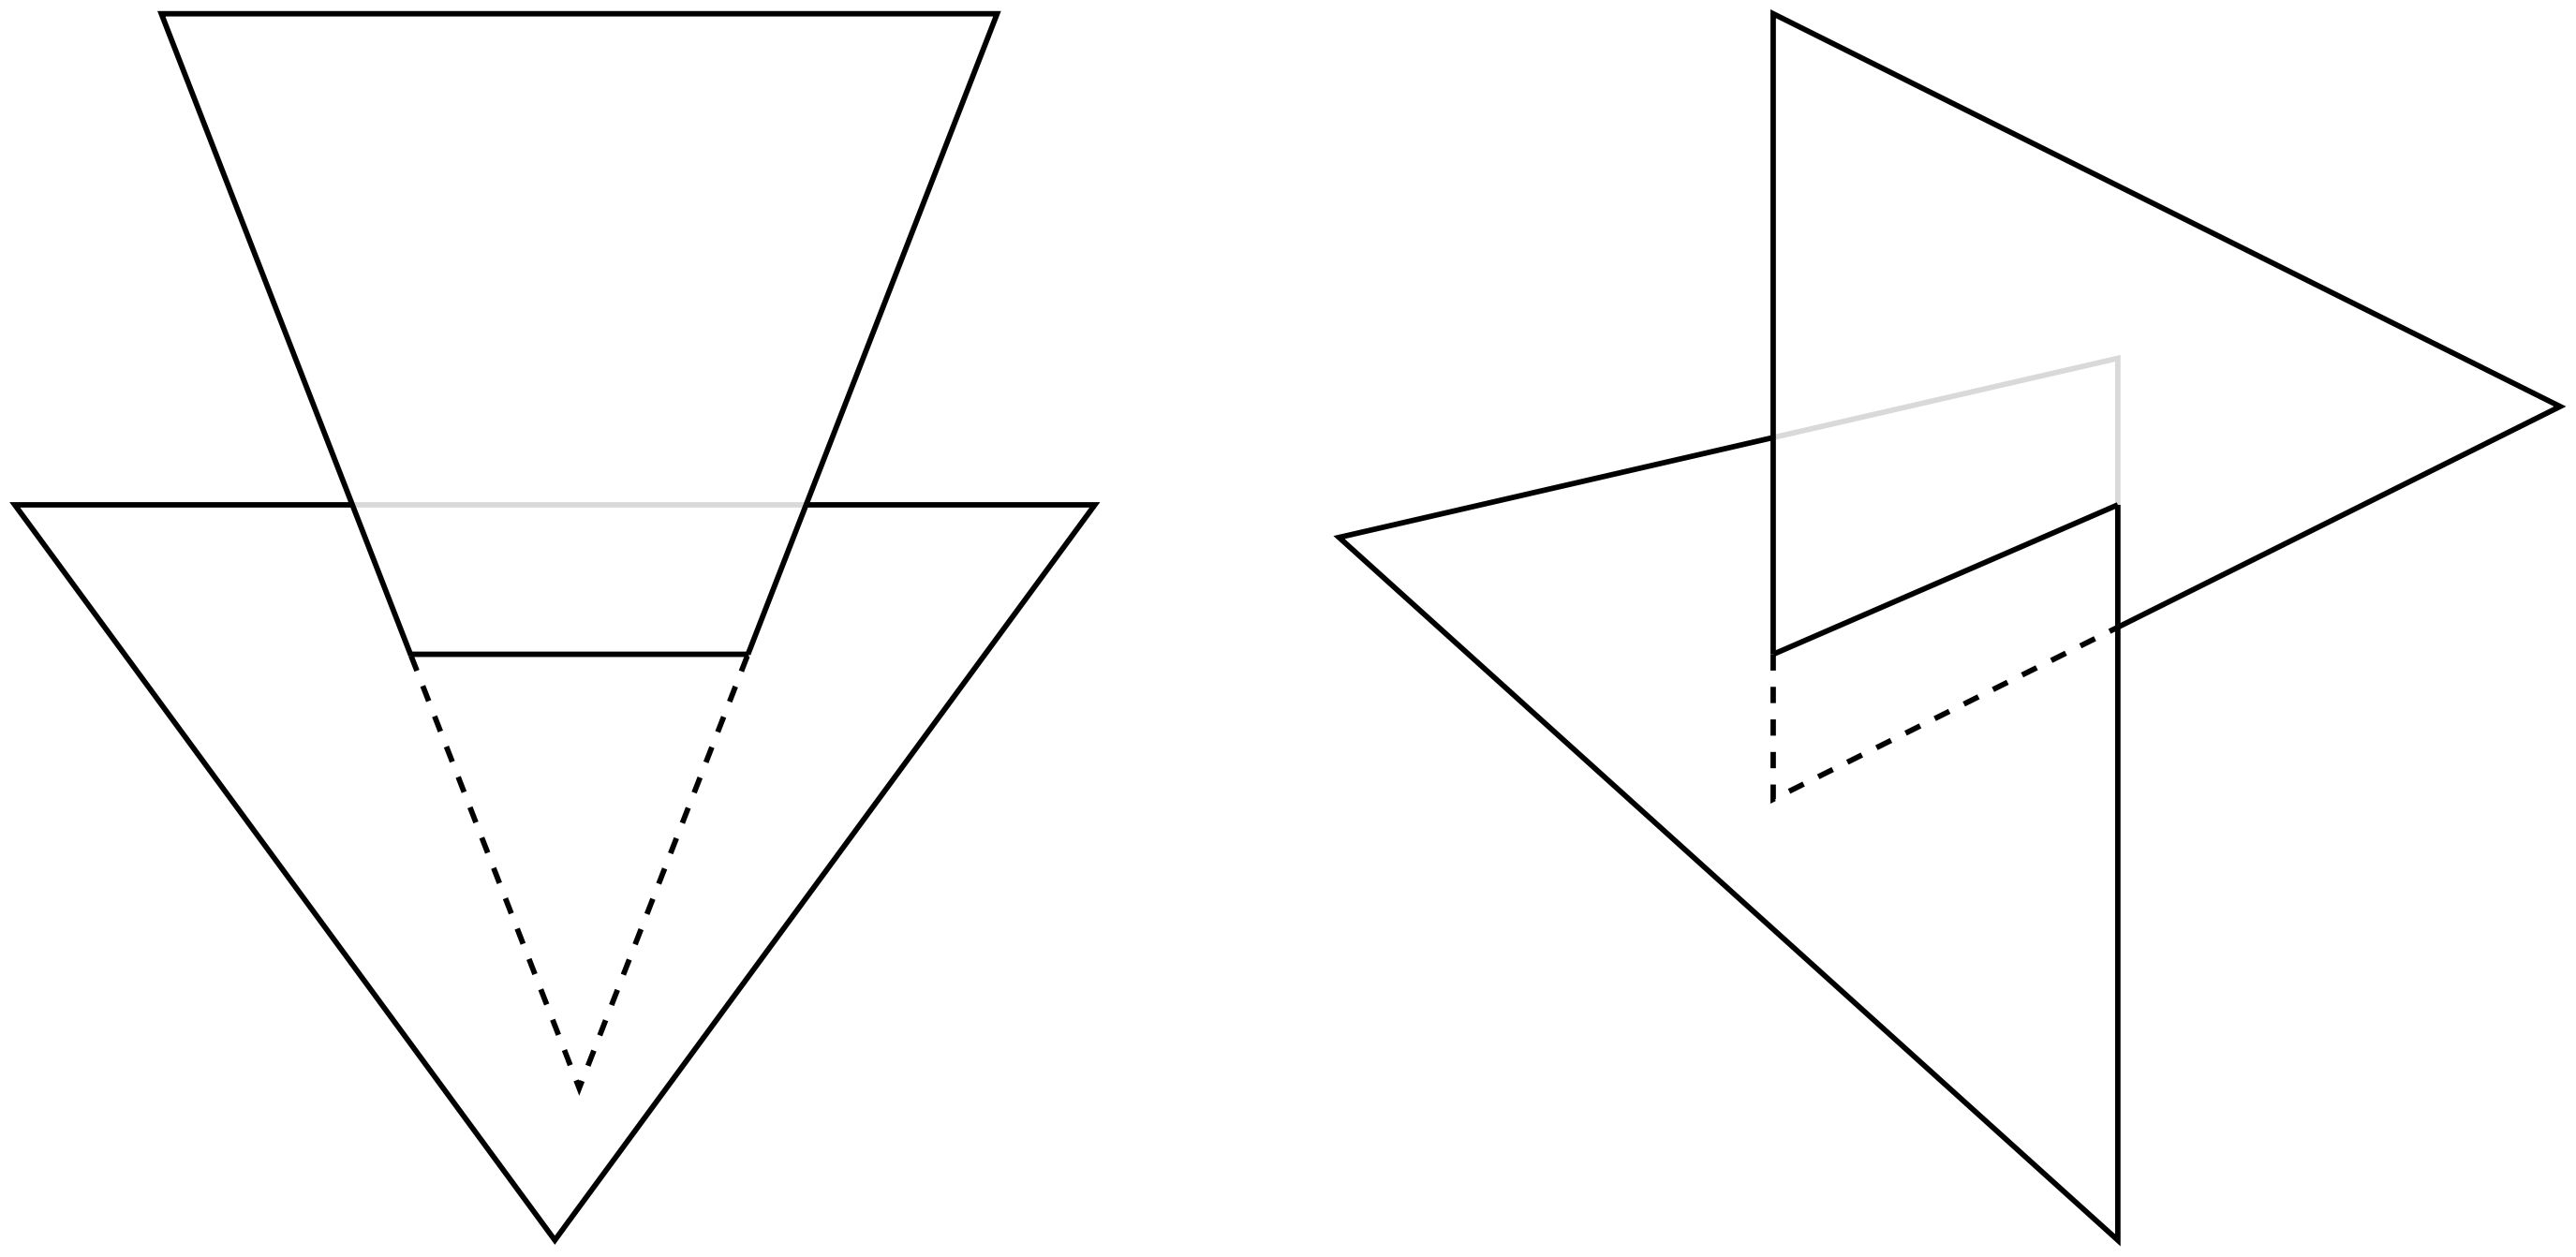
\includegraphics[width=0.8\textwidth]{pic/image-20231212174346327.png}
    \caption{两个三角形的相交情况}
    \label{fig:triangles}
\end{figure}

两个三角形相交:

\begin{itemize}[leftmargin=2cm]
    \item 要么一个三角形的两条边与另一个三角形相交(图\ref{fig:triangles}左侧)
    \item 或者两个三角形的一条边与另一个三角形相交(图\ref{fig:triangles}右侧)
\end{itemize}

步骤:检查第一个三角形的每一条边是否与第二个三角形相交,若有且仅有一条这样的边,说明两个三角形相交情况如图\ref{fig:triangles}右侧。若有两条边,说明相交情况如图\ref{fig:triangles}左侧。若没有这样的边,说明两个三角形不相交。

\section{}

\subsection{}

光线追踪:隐式表示。这是因为光线追踪中的相交测试通常涉及解方程,而使用隐式表示可以更容易地进行相交测试。通过将光线的参数代入椭球的隐式方程,我们可以判断是否有相交点。

光栅化:显式表示。这是因为在屏幕上的像素级别,使用显式表示更容易计算并进行图形渲染。显式表示可以直接转换为屏幕空间,而不需要解方程。

\subsection{}

由题意得,椭球的隐式方程为:

\[
    \frac{x^2}{a^2} + \frac{y^2}{b^2} + \frac{z^2}{c^2} = 1
\]

代入射线的参数方程,得到与射线的交点满足的方程:

\[
    \frac{\mathbf{o}_x+t\mathbf{d}_x}{a^2} + \frac{\mathbf{o}_y+t\mathbf{d}_y}{b^2} + \frac{\mathbf{o}_z+t\mathbf{d}_z}{c^2} = 1
\]

化简上述方程,得到关于$t$的二次方程。将其写成标准的二次方程形式$At^2+Bt+C=0$,其中:

\[
    % A = \frac{\mathbf{d}_x^2}{a^2} + \frac{\mathbf{d}_y^2}{b^2} + \frac{\mathbf{d}_z^2}{c^2}
    \begin{aligned}
        A & = \frac{\mathbf{d}_x^2}{a^2} + \frac{\mathbf{d}_y^2}{b^2} + \frac{\mathbf{d}_z^2}{c^2}                                  \\
        B & = 2(\frac{\mathbf{o}_x\mathbf{d}_x}{a^2} + \frac{\mathbf{o}_y\mathbf{d}_y}{b^2} + \frac{\mathbf{o}_z\mathbf{d}_z}{c^2}) \\
        C & = \frac{\mathbf{o}_x^2}{a^2} + \frac{\mathbf{o}_y^2}{b^2} + \frac{\mathbf{o}_z^2}{c^2} - 1
    \end{aligned}
\]

解这个二次方程,得到$t$的两个解。如果两个解都是正数,说明射线与椭球有两个交点;如果两个解都是负数,说明射线与椭球没有交点;如果有一个解是正数,一个解是负数,说明射线与椭球有一个交点。

\section{}

\begin{figure}
    \centering
    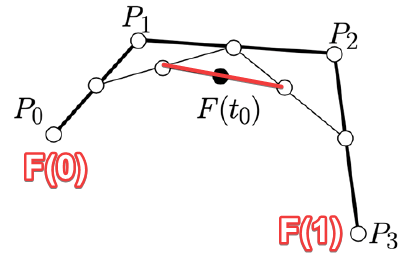
\includegraphics[width=0.8\textwidth]{pic/Acrobat_jD6Pv6U3E4.png}
    \caption{Answer 4}
    \label{fig:answer4}
\end{figure}

\subsection{}

$F(0)$和$F(1)$分别为图\ref{fig:answer4}中的$P_0$和$P_3$。

\subsection{}

$F$在$t$处$F(t)$的切线为图\ref{fig:answer4}中的红色线段。

\subsection{}

$P_3=G_0$,且线段$(P_2, P_3)$和$(G_0, G_1)$在同一条直线上。

\end{document}
